\PassOptionsToPackage{unicode=true}{hyperref} % options for packages loaded elsewhere
\PassOptionsToPackage{hyphens}{url}
%
\documentclass[ignorenonframetext,]{beamer}
\usepackage{pgfpages}
\setbeamertemplate{caption}[numbered]
\setbeamertemplate{caption label separator}{: }
\setbeamercolor{caption name}{fg=normal text.fg}
\beamertemplatenavigationsymbolsempty
\usepackage{lmodern}
\usepackage{amssymb,amsmath}
\usepackage{ifxetex,ifluatex}
\usepackage{fixltx2e} % provides \textsubscript
\ifnum 0\ifxetex 1\fi\ifluatex 1\fi=0 % if pdftex
  \usepackage[T1]{fontenc}
  \usepackage[utf8]{inputenc}
  \usepackage{textcomp} % provides euro and other symbols
\else % if luatex or xelatex
  \usepackage{unicode-math}
  \defaultfontfeatures{Ligatures=TeX,Scale=MatchLowercase}
\fi
\usetheme[]{CambridgeUS}
\usecolortheme{beaver}
\usefonttheme{structurebold}
% use upquote if available, for straight quotes in verbatim environments
\IfFileExists{upquote.sty}{\usepackage{upquote}}{}
% use microtype if available
\IfFileExists{microtype.sty}{%
\usepackage[]{microtype}
\UseMicrotypeSet[protrusion]{basicmath} % disable protrusion for tt fonts
}{}
\IfFileExists{parskip.sty}{%
\usepackage{parskip}
}{% else
\setlength{\parindent}{0pt}
\setlength{\parskip}{6pt plus 2pt minus 1pt}
}
\usepackage{hyperref}
\hypersetup{
            pdftitle={Overpass},
            pdfauthor={Jan-Philipp Kolb},
            pdfborder={0 0 0},
            breaklinks=true}
\urlstyle{same}  % don't use monospace font for urls
\newif\ifbibliography
\usepackage{color}
\usepackage{fancyvrb}
\newcommand{\VerbBar}{|}
\newcommand{\VERB}{\Verb[commandchars=\\\{\}]}
\DefineVerbatimEnvironment{Highlighting}{Verbatim}{commandchars=\\\{\}}
% Add ',fontsize=\small' for more characters per line
\usepackage{framed}
\definecolor{shadecolor}{RGB}{248,248,248}
\newenvironment{Shaded}{\begin{snugshade}}{\end{snugshade}}
\newcommand{\AlertTok}[1]{\textcolor[rgb]{0.94,0.16,0.16}{#1}}
\newcommand{\AnnotationTok}[1]{\textcolor[rgb]{0.56,0.35,0.01}{\textbf{\textit{#1}}}}
\newcommand{\AttributeTok}[1]{\textcolor[rgb]{0.77,0.63,0.00}{#1}}
\newcommand{\BaseNTok}[1]{\textcolor[rgb]{0.00,0.00,0.81}{#1}}
\newcommand{\BuiltInTok}[1]{#1}
\newcommand{\CharTok}[1]{\textcolor[rgb]{0.31,0.60,0.02}{#1}}
\newcommand{\CommentTok}[1]{\textcolor[rgb]{0.56,0.35,0.01}{\textit{#1}}}
\newcommand{\CommentVarTok}[1]{\textcolor[rgb]{0.56,0.35,0.01}{\textbf{\textit{#1}}}}
\newcommand{\ConstantTok}[1]{\textcolor[rgb]{0.00,0.00,0.00}{#1}}
\newcommand{\ControlFlowTok}[1]{\textcolor[rgb]{0.13,0.29,0.53}{\textbf{#1}}}
\newcommand{\DataTypeTok}[1]{\textcolor[rgb]{0.13,0.29,0.53}{#1}}
\newcommand{\DecValTok}[1]{\textcolor[rgb]{0.00,0.00,0.81}{#1}}
\newcommand{\DocumentationTok}[1]{\textcolor[rgb]{0.56,0.35,0.01}{\textbf{\textit{#1}}}}
\newcommand{\ErrorTok}[1]{\textcolor[rgb]{0.64,0.00,0.00}{\textbf{#1}}}
\newcommand{\ExtensionTok}[1]{#1}
\newcommand{\FloatTok}[1]{\textcolor[rgb]{0.00,0.00,0.81}{#1}}
\newcommand{\FunctionTok}[1]{\textcolor[rgb]{0.00,0.00,0.00}{#1}}
\newcommand{\ImportTok}[1]{#1}
\newcommand{\InformationTok}[1]{\textcolor[rgb]{0.56,0.35,0.01}{\textbf{\textit{#1}}}}
\newcommand{\KeywordTok}[1]{\textcolor[rgb]{0.13,0.29,0.53}{\textbf{#1}}}
\newcommand{\NormalTok}[1]{#1}
\newcommand{\OperatorTok}[1]{\textcolor[rgb]{0.81,0.36,0.00}{\textbf{#1}}}
\newcommand{\OtherTok}[1]{\textcolor[rgb]{0.56,0.35,0.01}{#1}}
\newcommand{\PreprocessorTok}[1]{\textcolor[rgb]{0.56,0.35,0.01}{\textit{#1}}}
\newcommand{\RegionMarkerTok}[1]{#1}
\newcommand{\SpecialCharTok}[1]{\textcolor[rgb]{0.00,0.00,0.00}{#1}}
\newcommand{\SpecialStringTok}[1]{\textcolor[rgb]{0.31,0.60,0.02}{#1}}
\newcommand{\StringTok}[1]{\textcolor[rgb]{0.31,0.60,0.02}{#1}}
\newcommand{\VariableTok}[1]{\textcolor[rgb]{0.00,0.00,0.00}{#1}}
\newcommand{\VerbatimStringTok}[1]{\textcolor[rgb]{0.31,0.60,0.02}{#1}}
\newcommand{\WarningTok}[1]{\textcolor[rgb]{0.56,0.35,0.01}{\textbf{\textit{#1}}}}
\usepackage{graphicx,grffile}
\makeatletter
\def\maxwidth{\ifdim\Gin@nat@width>\linewidth\linewidth\else\Gin@nat@width\fi}
\def\maxheight{\ifdim\Gin@nat@height>\textheight\textheight\else\Gin@nat@height\fi}
\makeatother
% Scale images if necessary, so that they will not overflow the page
% margins by default, and it is still possible to overwrite the defaults
% using explicit options in \includegraphics[width, height, ...]{}
\setkeys{Gin}{width=\maxwidth,height=\maxheight,keepaspectratio}
% Prevent slide breaks in the middle of a paragraph:
\widowpenalties 1 10000
\raggedbottom
\setbeamertemplate{part page}{
\centering
\begin{beamercolorbox}[sep=16pt,center]{part title}
  \usebeamerfont{part title}\insertpart\par
\end{beamercolorbox}
}
\setbeamertemplate{section page}{
\centering
\begin{beamercolorbox}[sep=12pt,center]{part title}
  \usebeamerfont{section title}\insertsection\par
\end{beamercolorbox}
}
\setbeamertemplate{subsection page}{
\centering
\begin{beamercolorbox}[sep=8pt,center]{part title}
  \usebeamerfont{subsection title}\insertsubsection\par
\end{beamercolorbox}
}
\AtBeginPart{
  \frame{\partpage}
}
\AtBeginSection{
  \ifbibliography
  \else
    \frame{\sectionpage}
  \fi
}
\AtBeginSubsection{
  \frame{\subsectionpage}
}
\setlength{\emergencystretch}{3em}  % prevent overfull lines
\providecommand{\tightlist}{%
  \setlength{\itemsep}{0pt}\setlength{\parskip}{0pt}}
\setcounter{secnumdepth}{0}

% set default figure placement to htbp
\makeatletter
\def\fps@figure{htbp}
\makeatother


\title{Overpass}
\author{Jan-Philipp Kolb}
\date{23 Oktober 2018}

\begin{document}
\frame{\titlepage}

\begin{frame}{Themen dieses Abschnitts}
\protect\hypertarget{themen-dieses-abschnitts}{}

\begin{itemize}
\tightlist
\item
  Die
  \href{https://wiki.openstreetmap.org/wiki/Overpass_API}{\textbf{Overpass
  API}} von Roland Olbricht wird vorgestellt.
\item
  Die API \href{https://overpass-turbo.eu/}{\textbf{Overpass Turbo}}
\item
  Wie man die OSM Daten graphisch darstellen kann.
\end{itemize}

\end{frame}

\begin{frame}{Die Overpass API}
\protect\hypertarget{die-overpass-api}{}

\begin{itemize}
\tightlist
\item
  Die von Roland Olbricht geschriebene Overpass API ermöglicht es
  Entwicklern, kleine Auszüge von benutzergenerierten Inhalten von
  Openstreetmap nach vorgegebenen Kriterien herunterzuladen.
\item
  Overpass ist eine read-only API, die durch den Benutzer ausgewählte
  Teile der OSM-Daten bereitstellt.
\item
  Overpass kann als eine Datenbank über das Internet verstanden werden.
\item
  Die API eignet sich besonders gut, wenn man nach ganz speziellen Map
  Features sucht.
\end{itemize}

\end{frame}

\begin{frame}{\href{https://overpass-turbo.eu/}{Overpass Turbo}}
\protect\hypertarget{overpass-turbo}{}

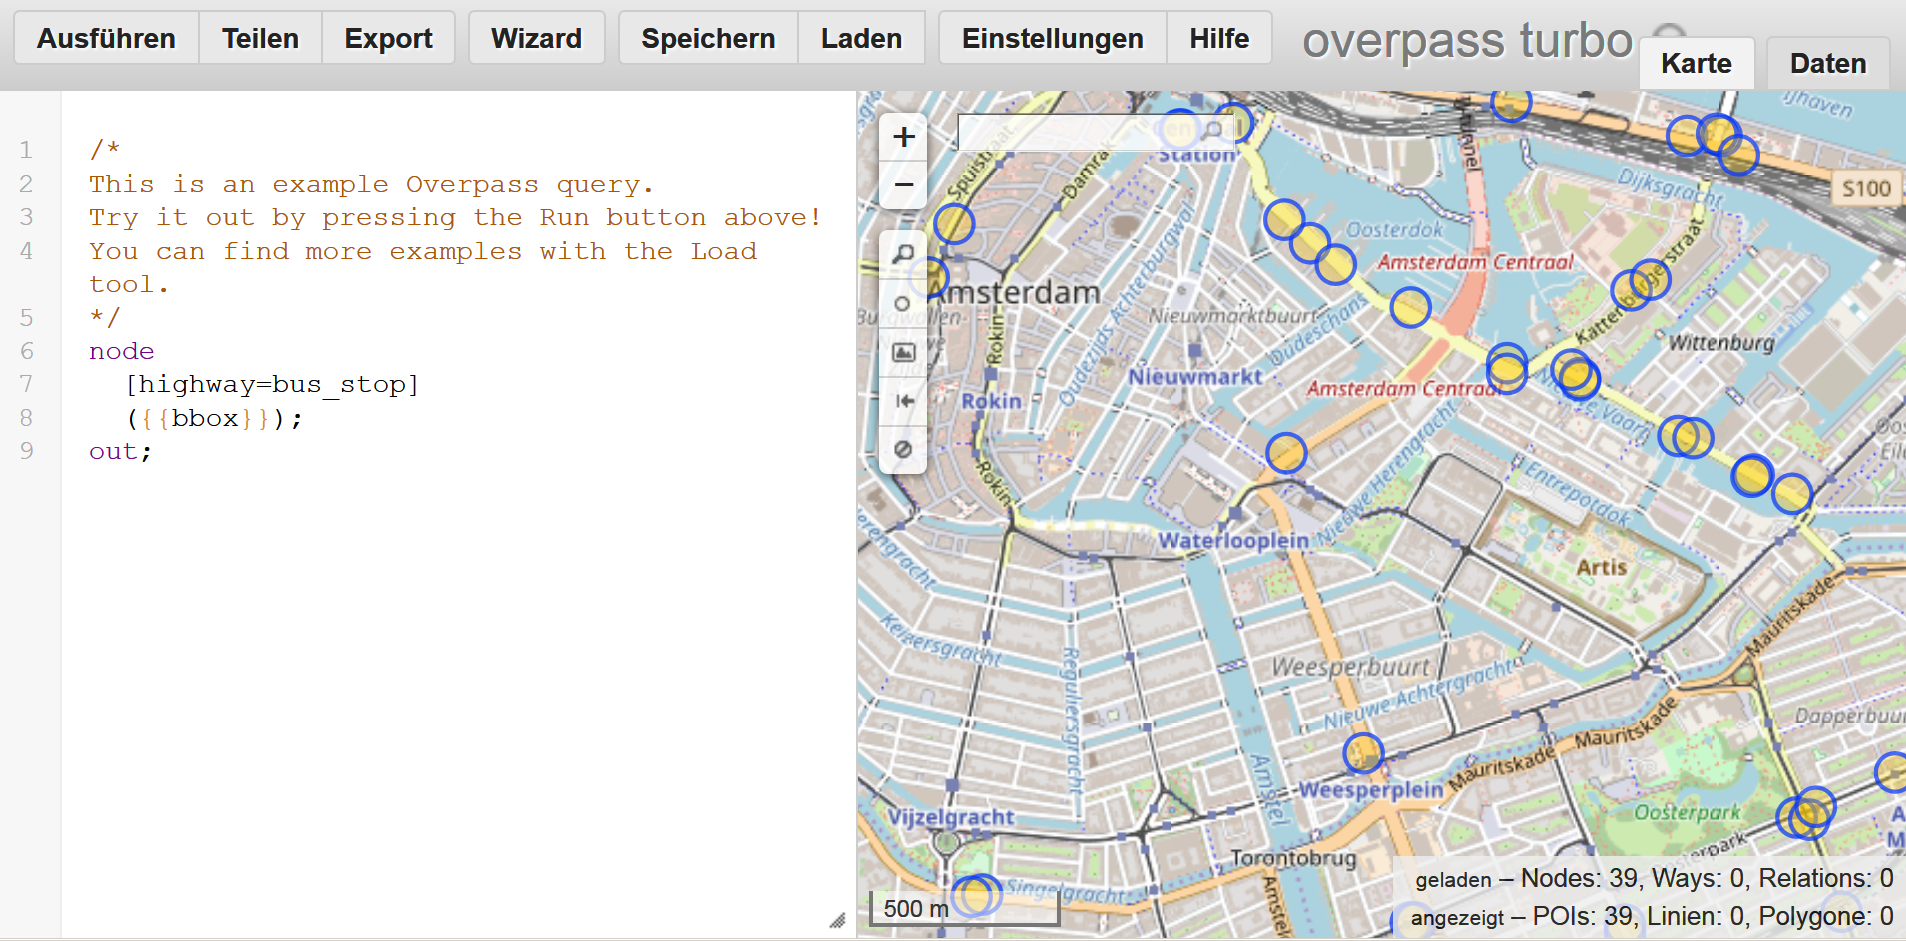
\includegraphics{figure/overpassTurbo.PNG}

\end{frame}

\begin{frame}[fragile]{Query Overpass}
\protect\hypertarget{query-overpass}{}

\begin{itemize}
\tightlist
\item
  In der folgenden Abfrage wird bei Overpass Turbo nach Bars im
  ausgewählten Fenster gesucht.
\end{itemize}

\begin{verbatim}
node
  [amenity=bar]
  ({{bbox}});
out;
\end{verbatim}

\end{frame}

\begin{frame}{Export bei Overpass}
\protect\hypertarget{export-bei-overpass}{}

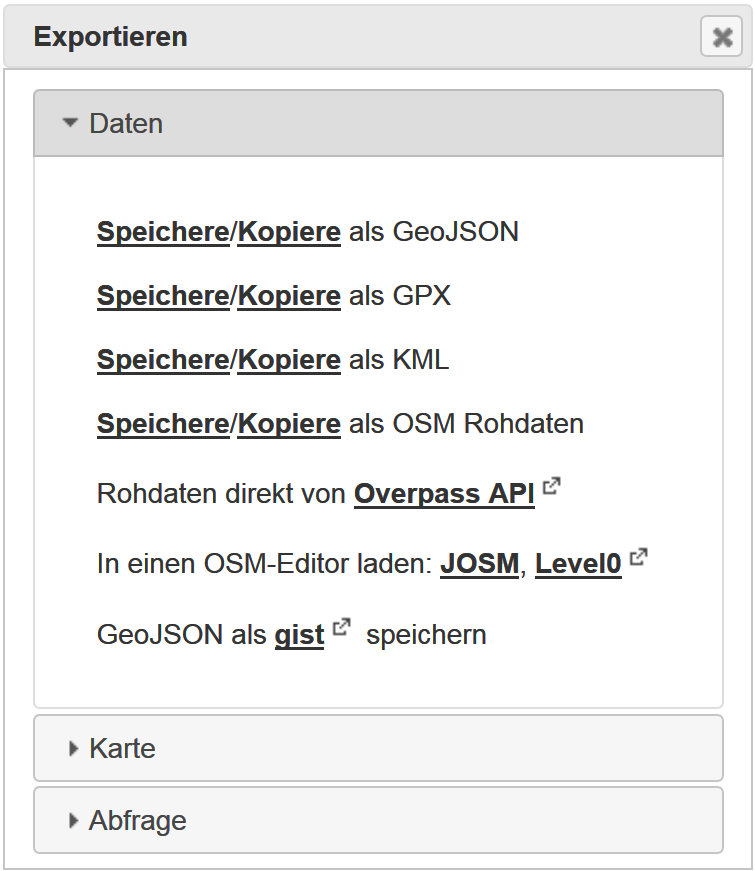
\includegraphics{figure/OverpassExport.PNG}

\end{frame}

\begin{frame}{Speicherformate}
\protect\hypertarget{speicherformate}{}

\begin{block}{Bei Export von Overpass}

\begin{itemize}
\tightlist
\item
  GeoJSON
\item
  GPX
\item
  KML
\item
  OSM Rohdaten
\end{itemize}

\end{block}

\end{frame}

\begin{frame}[fragile]{Import von Daten}
\protect\hypertarget{import-von-daten}{}

\begin{Shaded}
\begin{Highlighting}[]
\KeywordTok{library}\NormalTok{(XML)}
\NormalTok{dat <-}\StringTok{ }\KeywordTok{xmlParse}\NormalTok{(}\StringTok{"../data/bus_stop_amsterdam.kml"}\NormalTok{)}
\end{Highlighting}
\end{Shaded}

\begin{Shaded}
\begin{Highlighting}[]
\NormalTok{xmltop <-}\StringTok{ }\KeywordTok{xmlRoot}\NormalTok{(dat)}
\NormalTok{xmltop[[}\DecValTok{1}\NormalTok{]][[}\DecValTok{1}\NormalTok{]]}
\end{Highlighting}
\end{Shaded}

\begin{verbatim}
## <name>overpass-turbo.eu export</name>
\end{verbatim}

\end{frame}

\begin{frame}[fragile]{Xpath Abfragesprache}
\protect\hypertarget{xpath-abfragesprache}{}

\begin{block}{Beispiel: \href{https://de.wikipedia.org/wiki/XPath}{xpath
wikipedia}}

\begin{Shaded}
\begin{Highlighting}[]
\KeywordTok{xpathApply}\NormalTok{(dat,}\StringTok{"Document"}\NormalTok{)}
\end{Highlighting}
\end{Shaded}

\begin{verbatim}
## list()
## attr(,"class")
## [1] "XMLNodeSet"
\end{verbatim}

\end{block}

\end{frame}

\begin{frame}[fragile]{JSON importieren}
\protect\hypertarget{json-importieren}{}

\begin{Shaded}
\begin{Highlighting}[]
\KeywordTok{install.packages}\NormalTok{(}\StringTok{"rjson"}\NormalTok{)}
\KeywordTok{library}\NormalTok{(rjson)}
\end{Highlighting}
\end{Shaded}

\begin{Shaded}
\begin{Highlighting}[]
\KeywordTok{library}\NormalTok{(jsonlite)}
\NormalTok{dat<-jsonlite}\OperatorTok{::}\KeywordTok{fromJSON}\NormalTok{(}\StringTok{"../data/amsterdam_busstop.geojson"}\NormalTok{)}
\KeywordTok{typeof}\NormalTok{(dat)}
\end{Highlighting}
\end{Shaded}

\begin{verbatim}
## [1] "list"
\end{verbatim}

\begin{Shaded}
\begin{Highlighting}[]
\KeywordTok{names}\NormalTok{(dat)}
\end{Highlighting}
\end{Shaded}

\begin{verbatim}
## [1] "type"      "generator" "copyright" "timestamp" "features"
\end{verbatim}

\end{frame}

\begin{frame}[fragile]{Wie sehen die Daten aus}
\protect\hypertarget{wie-sehen-die-daten-aus}{}

\begin{Shaded}
\begin{Highlighting}[]
\NormalTok{DT}\OperatorTok{::}\KeywordTok{datatable}\NormalTok{(dat}\OperatorTok{$}\NormalTok{features}\OperatorTok{$}\NormalTok{properties)}
\end{Highlighting}
\end{Shaded}

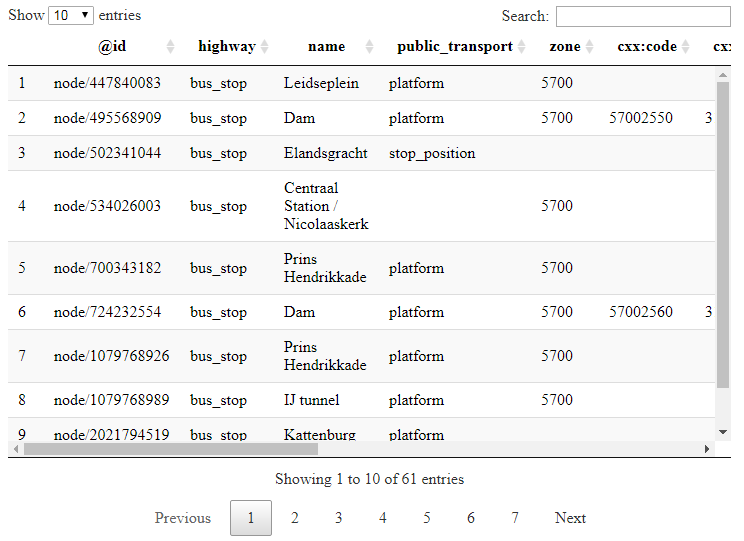
\includegraphics{figure/amsterdam_busstop_features.PNG}

\end{frame}

\begin{frame}[fragile]{GPX file importieren}
\protect\hypertarget{gpx-file-importieren}{}

\begin{Shaded}
\begin{Highlighting}[]
\KeywordTok{library}\NormalTok{(plotKML)}
\end{Highlighting}
\end{Shaded}

\begin{verbatim}
## plotKML version 0.5-8 (2017-05-12)
\end{verbatim}

\begin{verbatim}
## URL: http://plotkml.r-forge.r-project.org/
\end{verbatim}

\begin{Shaded}
\begin{Highlighting}[]
\NormalTok{dat_gpx <-}\StringTok{ }\KeywordTok{readGPX}\NormalTok{(}\StringTok{"../data/Amsterdam_busstop.gpx"}\NormalTok{)}
\KeywordTok{head}\NormalTok{(dat_gpx}\OperatorTok{$}\NormalTok{waypoints)}
\end{Highlighting}
\end{Shaded}

\begin{verbatim}
##        lon      lat                            name
## 1 4.880870 52.36213                     Leidseplein
## 2 4.891237 52.37438                             Dam
## 3 4.877558 52.36953                    Elandsgracht
## 4 4.900331 52.37670 Centraal Station / Nicolaaskerk
## 5 4.905498 52.37395               Prins Hendrikkade
## 6 4.890181 52.37310                             Dam
##                                                                                                                            desc
## 1                                                      highway=bus_stop\nname=Leidseplein\npublic_transport=platform\nzone=5700
## 2                 cxx:code=57002550\ncxx:id=31843\nhighway=bus_stop\nname=Dam\npublic_transport=platform\nsource=CXX\nzone=5700
## 3                     bus=yes\nhighway=bus_stop\nname=Elandsgracht\npublic_transport=stop_position\nrailway=tram_stop\ntram=yes
## 4                            bench=yes\nbin=yes\nhighway=bus_stop\nname=Centraal Station / Nicolaaskerk\nshelter=yes\nzone=5700
## 5 bench=yes\nbin=yes\nhighway=bus_stop\nname=Prins Hendrikkade\noperator=GVB\npublic_transport=platform\nshelter=yes\nzone=5700
## 6        bus=yes\ncxx:code=57002560\ncxx:id=31844\nhighway=bus_stop\nname=Dam\npublic_transport=platform\nsource=CXX\nzone=5700
##   link
## 1     
## 2     
## 3     
## 4     
## 5     
## 6
\end{verbatim}

\end{frame}

\end{document}
